\chapter{版式}

本文使用的长度单位:
1英寸 = 25.4mm = 72.27pt \footnote{pt是point的缩写,中文叫“磅”。} = 72bp。
注意 \TeX 定义的pt和PostScript(亦即Adobe系列软件)定义的pt的长度不一样,
本书以 \TeX 定义的pt为准,Post\-Script的基本长度单位写为bp(big point)。

\section{纸张大小} %%%%%%%%%%%%%%%%%%%%%%%%%%%%%%

书籍的纸张大小通常异于常用的打印纸大小(A4或B5),
因此用 \LaTeX 排版书籍的第一步是设置好纸张大小。
一般常见的IT图书的开本(成品书尺寸,可以用尺子量出来)是 185mm $\times$ 230mm,
即“国际18开”;另外一种常见开本是185mm $\times$ 260mm,即“16开”。
本文以“国际18开”为例。
我们通常可以用 \fn{geometry} 宏包来设置纸张和版心尺寸,
例子见 \S \ref{sec:textbody}。
\index{宏包!geometry@\fn{geometry}|(}
%\index{开本}

\section{版心大小} %%%%%%%%%%%%%%%%%%%%%%%%%%%%%%
\label{sec:textbody}

“版心”即正文区,不包含页眉和页脚
\footnote{这是本文的定义,也有将版心定义为包含页眉和页脚的。}。
版心的大小可以这样计算:
通常正文字号是10pt
\footnote{比五号(10.5pt)字略小,比小五号字(9pt)大。},
一行按39个汉字计算,
%\footnote{。一般不宜超过40个。}
那么行宽是 390pt。
行宽是正文字号的整数倍,这样中文间距不会无故拉宽。
行宽不宜过大,否则阅读的时候容易读串行;
也不宜过小,否则一行排不下80列代码。一般而言,
36 \textasciitilde\ 42字比较适宜,本文定为39字,数数上一行:-)。
\mybooktitle 一行是37个汉字,
因为这本书厚达600页,如果版心太宽容易影响阅读订口的文字。

对于10pt的正文字体,\LaTeX 默认的行距
\footnote{行距指的是英文基线(baseline)之间的距离,即中文汉字底部之间的距离,
不是两行之间的空白。} 是12pt,这对于英文是合适的
\footnote{因为英文文本多是小写字母,字高远小于10pt。},
但是对于中文则显得太密了。因此 \CTeX 宏包将 \mn{baselinestretch} 定义为 1.3,
\index{命令!baselinestretch@\mn{baselinestretch}}
这样行距是\linebreak 1.3$\times$12pt = 15.6pt,阅读起来就比较顺眼了。
如果一页排34行字,那么版心的高度大约是 \nolinebreak
\footnote{这里说“大约”,因为第一行上方似乎不必留出多余的空白。} 34$\times$15.6pt=530.4pt,
本文取 530pt
\footnote{对于技术类图书,通常一个自然段不会太长,
一页之内几乎总是会遇到分段(整段代码、图表、章节标题)的情况,
因此版心高度不必严格是行距的整数倍。} 。

综上,对于39字 $\times$ 34行的版心,其尺寸是 390pt $\times$ 530pt,约合 137mm $\times$ 186mm。见下图示意。

%\vspace{1ex}
\centerline{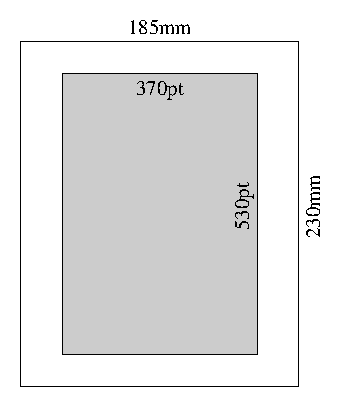
\includegraphics{paper.eps}}

知道了纸张和版心尺寸,剩下的就交给 \fn{geometry} 宏包。
它同时会设置生成的PDF的纸张尺寸。
例如 \myurl{examples/paper.tex}。
\index{宏包!geometry@\fn{geometry}|)}

\begin{Codex}[label=examples/paper.tex]
\documentclass[10pt,fancyhdr,UTF8]{ctexbook}
\usepackage[centering,paperwidth=180mm,paperheight=230mm,%
            body={390pt,530pt},showframe]{geometry}
\end{Codex}

注意这里把纸张宽度设为 180mm,这是考虑到装订的位置,
这样在电脑上预览的时候左右空白更贴近实际印刷的效果。
我们也不必关心版心在纸张中的上下左右位置,居中即可,
在印刷的时候有专人负责拼版。当然在正式排版的时候要去掉 \fn{showframe} 选项。

另外,打印纸一般不会刚好和书籍开本一样大,
要想在书印出来之前感受版面效果,
可以打印在A4纸上,但需要将书页框出来,可用 \fn{crop} 宏包。
例如 \myurl{examples/paper-crop.tex}。
\index{宏包!crop@\fn{crop}}

\begin{Code}
$ diff -u paper.tex paper-crop.tex
--- paper.tex           2012-12-29 14:03:02.000 +0800
+++ paper-crop.tex      2012-12-29 14:03:02.000 +0800
 \documentclass[10pt,fancyhdr,UTF8]{ctexbook}
 \usepackage[centering,paperwidth=180mm,paperheight=230mm,%
             body={390pt,530pt},showframe]{geometry}
+\usepackage[a4,center,frame,color=blue]{crop}
\end{Code}

\section{页眉与页脚} %%%%%%%%%%%%%%%%%%%%%%%%%%%%%%

书籍排版不是以一页(一面)为单位,而是以翻开之后的两面(左右页)为单位。
\LaTeX 默认会设法让左右页的内容一样多,即左右页的最后一行位于同一高度。
有时候这会造成难看的版面,特别是有可能留下过多段间空白。
一般可以用 \mn{raggedbottom} 命令来取消这一设定。
\index{命令!raggedbottom@\mn{raggedbottom}}

页眉的外侧(切口)是页码,内侧(订口)是章节名称,通常是左页(偶数页)放章名,
右页(奇数页)放节名
\footnote{\mybooktitle p.393 的内侧页眉为空,因为该章第1节出现在 p.394。}。
页脚通常可以放书名,这样即便复印其中一面也容易知道出自何处%
(本文把作者姓名和网址也放到页脚,便于网上传播)。
典型的安排如下图所示。

\vspace{1ex}
\centerline{\fbox{
\includegraphics[page=2,scale=0.9]{header.pdf}}%
\quad\fbox{
\includegraphics[page=3,scale=0.9]{header.pdf}}}

\vspace{1ex}
我们一般用 \fn{fancyhdr} 宏包来设置页眉和页脚,常用的设置如下。
其中 \fn{RE} 表示偶数页\linebreak(Even)右侧(Right),
\fn{LO} 表示奇数页(Odd)左侧(Left),
\fn{LE}、\fn{RO} 的意思想必读者能举一反三猜出来。
\index{宏包!fancyhdr@\fn{fancyhdr}}

\begin{Code}
\pagestyle{fancy}
\fancyhf{}
\fancyhead[RE]{\normalfont\small\rmfamily\nouppercase{\leftmark}}
\fancyhead[LO]{\normalfont\small\rmfamily\nouppercase{\rightmark}}
\fancyhead[LE,RO]{\thepage}
\fancyfoot[LE,LO]{\small Book Title}
\end{Code}

通常每章的第一页没有页眉,页码放到页脚中央,即 \fn{plain} 页面格式,如下图所示。

\vspace{1ex}
\centerline{\fbox{
\includegraphics[page=1,scale=0.9]{header.pdf}}}

\section{中文字体} %%%%%%%%%%%%%%%%%%%%%%%%%%%%%%

首先,适合屏幕阅读的字体不一定适合印刷书籍。
原因可能有两点,一是书籍的印刷分辨率远高于屏幕;
二是屏幕会主动发光,而书籍是被动反光。
其次,中文字体用三四种(宋、黑、楷)就足够了,不要太花哨。
印刷用的正文字体可用方正书宋或华康简宋,
视出版社的字体授权情况而定。
屏幕阅读可用Windows中文字体或Adobe中文字体。
注意某些Adobe中文字体的标点符号位置不正确,
例如Adobe楷体的全角冒号和分号上下居中,而不是位于左下角(
\setCJKfamilyfont{adobekai}{Adobe Kaiti Std}
{\CJKfamily{adobekai}子曰:“食不厌精;脍不厌细。”}),
使用时需要注意。
另外,方正书宋和华康简宋缺少某些繁体字(例如“碁”),可以临时改换为Adobe宋体。
例如
\begin{Code}
\setCJKfamilyfont{adobesong}{Adobe Song Std}
《C++编程规范(繁体版)》由{\CJKfamily{adobesong} 碁峰}出版社出版。
\end{Code}

\subsection{不要使用中文斜体}
\label{subsec:noChineseItalic}
中文斜体是非常难看的,千万不要用。
为了突出中文术语,可以用\textbf{黑体},例如\textbf{与非门}。
传统科技书籍也常用{\kaishu 楷体}表示术语和强调,不过黑体目前似乎更流行一些。


\section{英文字体} %%%%%%%%%%%%%%%%%%%%%%%%%%%%%%
英文字体可选择的范围就大多了,可参考
The \LaTeX\ Font Catalogue \footnote{\myurl{http://www.tug.dk/FontCatalogue/}}。

\subsection{罗马字体}
不要使用 {\fontfamily{lmr}\selectfont Computer Modern Roman},
它笔画太细而且衬线略显夸张。
英文罗马字体一般可以选 {\fontspec{Times New Roman} Times Roman} 
\footnote{实际的字体名是 \fn{Nimbus Roman No9 L} 或 \fn{TeX Gyre Termes} 或 \fn{Times New Roman} 等。}
或 {\fontspec{URW Palladio L} Palatino}
\footnote{实际的字体名是 \fn{URW Palladio L} 或 \fn{TeX Gyre Pagella} 等。}。
例如
\begindot
\item {\fontspec{TeX Gyre Termes} C++ is a general-purpose programming language. [Times Roman]}
\item {\fontspec{TeX Gyre Pagella} C++ is a general-purpose programming language. [Palatino]}
\myenddot

\subsection{无衬线字体}

一般用于章节标题和编程语言关键字,例如“\kw{this} 指针”、
“\kw{mutable} 成员变量”。由于它出现的机会少,用什么字体其实无所谓,
默认的 \kw{Computer Modern Sans Serif} 就行。
也可以换为 {\fontspec{Nimbus Sans L} Helvetica} 
\footnote{实际的字体名是 \fn{Nimbus Sans L} 或 \fn{TeX Gyre Heros} 或 \fn{Arial} 等。}。

\subsection{等宽字体}
一般用于代码,包括变量名、类名等等。
不要使用 {\fontspec{Courier New} Courier New},它太细而且太宽。
可以用\LaTeX 默认的 {\fontspec{Latin Modern Mono} Computer Modern Typewriter}
\footnote{实际字体名是 \fn{Latin Modern Mono}。} 
或 {\fontspec{Inconsolata} Inconsolata}。后者要窄一些,但是双引号略弯。例如
\begindot
\item[] {\small \fontspec{Latin Modern Mono} printf("Hello \%s\bs n", name);} [cmtt]
\item[] {\small \fontspec[Mapping=tex-text-tt]{Inconsolata} printf("Hello \%s\bs n", name);} [Inconsolata]
\myenddot

注意如果要使用 Inconsolata 字体来排版代码,需要防止 \LaTeX 替换其中的字符,
例如 {\fontspec[Mapping=tex-text-tt]{Inconsolata} operator<<()} 变成 {\fontspec{Inconsolata} operator<<()} 等。
可以通过 \fn{fontspec} 宏包的 \fn{Mapping} 选项来做到这一点,
并搭配合适的 TECkit 映射文件
\footnote{见本文源码目录中的 \fn{tex-text-tt.map},需要用 \fn{teckit_compile} 工具编译为 \fn{{}.tec} 文件。}。

如果要排版大量Java代码(一行可长达100列),可以考虑用窄的无衬线等宽字体,
如 TheSansMono Condensed,但似乎没有免费版本。
另外,一些英文书籍也用 {\small \fontspec{Lucida Sans Typewriter}Lucida Sans Typewriter} 来排版代码,可以从Sun JDK中找到。

\subsection{特殊字体}
URL可以用窄字体,以节省空间。
例如 {\fontspec{Ubuntu Condensed}Ubuntu Condensed} 或者 \myurl{PT Sans Narrow}。
特殊术语可以用稍微夸张一点的字体凸显,例如“{\fontspec{URW Gothic L} Extract Method} 重构”和
“{\fontspec{URW Gothic L} Observer} 模式”。

\section{行距与段距}
中文区分自然段的方法有三种,传统的方案是段首空两格(indent),
现代的方案是两段之间增加空白(\mn{parskip}),
第三种方案是同时使用前两者。本文采用传统方案,
\mybooktitle 一书采用第三种方案。
设置\mn{parskip} 的时候要小心,它会影响所有段落之前的空白,
包括章节标题、图表、图表编号等等。
\index{命令!parskip@\mn{parskip}}

\section{整段代码}
\index{宏包!fancyvrb@\fn{fancyvrb}}
用等宽字体排版代码一般可用 \fn{fancyvrb} 宏包,然后定义自己的\fn{Code} 环境,
字号9pt,行距0.9,左边留出3mm。
\begin{Code}
\DefineVerbatimEnvironment{Code}{Verbatim}%
  {fontsize=\small,baselinestretch=0.9,xleftmargin=3mm}
\end{Code}

用 {\fontspec{Latin Modern Mono} Computer Modern Typewriter} 字体,版心宽度390pt时,一行可排80列。
\begin{Verbatim}[fontsize=\small,baselinestretch=0.9,xleftmargin=3mm]
\begin{Code}
12345678901234567890123456789012345678901234567890123456789012345678901234567890
         1         2         3         4         5         6         7         8
\end{Code}
\end{Verbatim}

用 {\fontspec{Inconsolata} Inconsolata} 字体,版心宽度为390pt时,一行可排84列。
版心宽度为370pt时可排80列。
%\setmonofont[AutoFakeBold=1.6,AutoFakeSlant=0.17,Mapping=tex-text-tt]{Inconsolata}
\makeatletter
\@namedef{FV@fontfamily@inconsolata}{%
  \def\FV@FontScanPrep{}%
  \def\FV@FontFamily{\fontspec{Inconsolata}}}
\makeatother
\begin{Code}[fontfamily=inconsolata]
123456789012345678901234567890123456789012345678901234567890123456789012345678901234
         1         2         3         4         5         6         7         8
\end{Code}

另外还可以定义\fn{Codex} 环境,用于排版带标题(文件名)的代码。

\begin{Code}
\DefineVerbatimEnvironment{Codex}{Verbatim}%
  {fontsize=\small,baselinestretch=0.9,xleftmargin=3mm,%
  frame=lines,labelposition=all,framesep=5pt}
\end{Code}

我对 \fn{fancyvrb} 宏包有一些改动,见 \fn{verbatim.cls}。
最终效果如下:
\begin{Codex}[label=hello.c,numbers=left]
int main()
{
  printf("Hello, world.\n");
}
\end{Codex}
